\section{时空端到端应用}
\subsection{联合检测和数据关联的实时在线多目标跟踪方案}

\begin{frame}{端到端网络设计的动机}
	\begin{figure}[!t]
		\centering
		\includegraphics[width=3.7in]{../figures/C5Fig/consistency.pdf}
		\caption{两阶段、一阶段和端到端方法的对比}
	\end{figure}
\end{frame}


\begin{frame}{联合检测关联的网络架构图}
	\begin{figure}[!t]
		\centering
		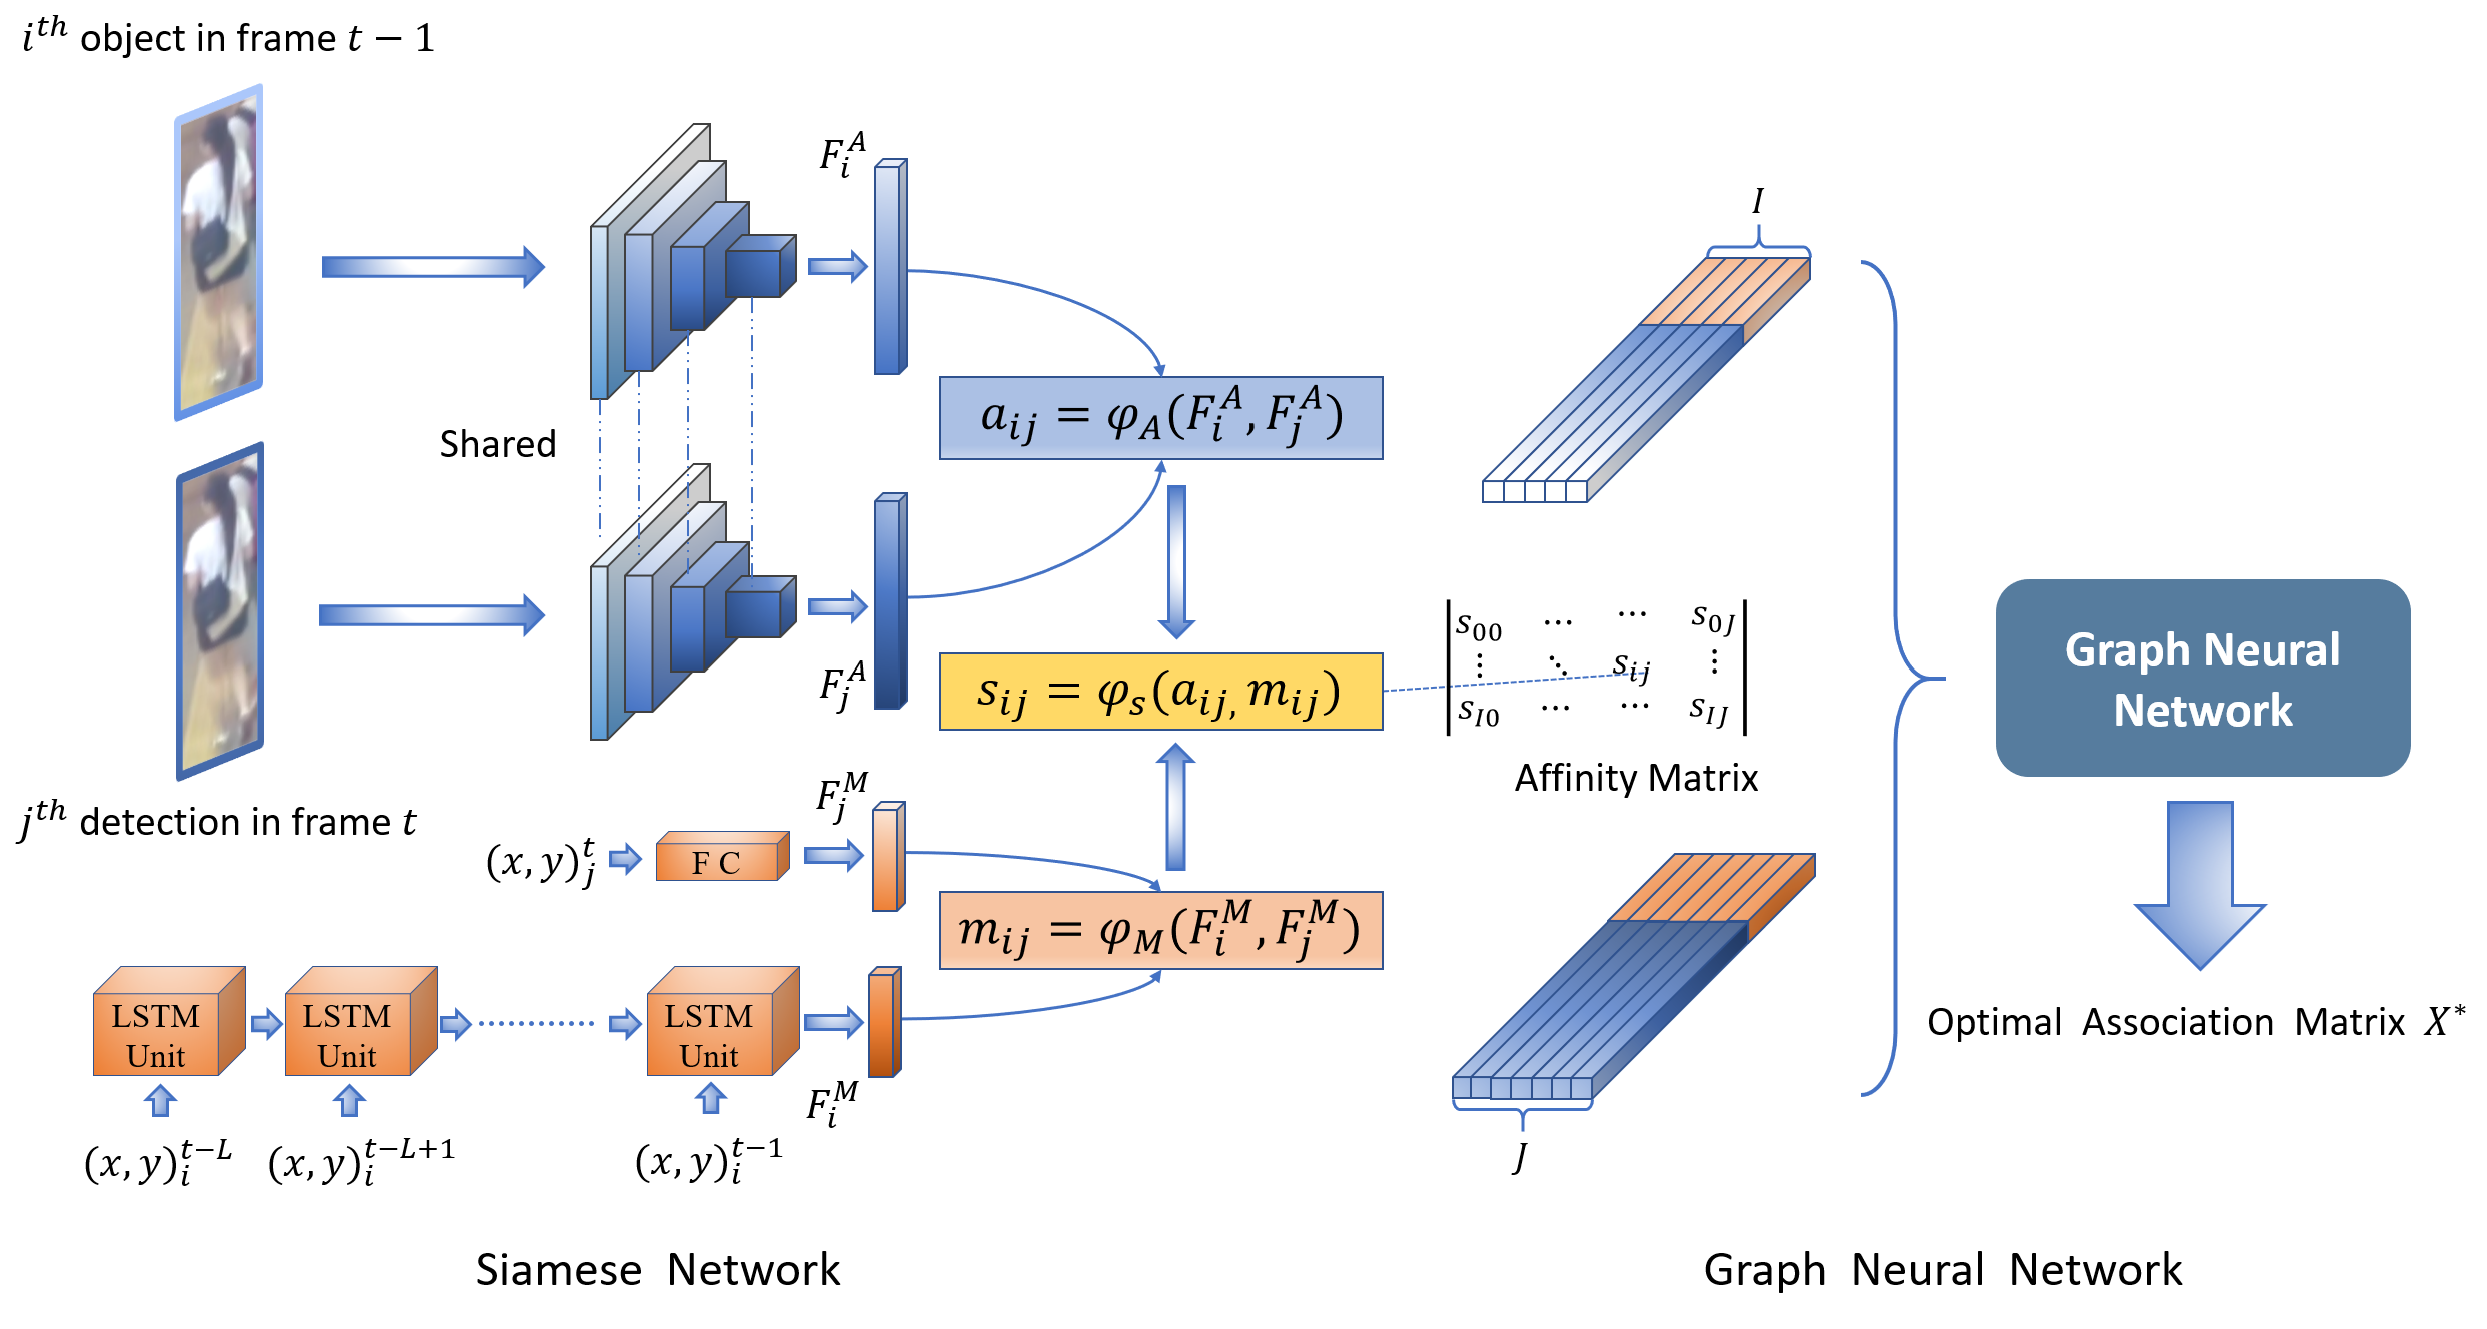
\includegraphics[width=4.5in]{../figures/C5Fig/pipeline.pdf}
%		\caption{两阶段、一阶段和端到端方法的对比}
	\end{figure}
\end{frame}


\begin{frame}{损失函数的设计}
	\begin{figure}[!t]
		\centering
		\includegraphics[width=4.5in]{../figures/C5Fig/loss.pdf}
		\caption{目标消失和出现的处理}
	\end{figure}
\end{frame}


\begin{frame}{端到端跟踪}
	\begin{figure}[!t]
		\centering
		\includegraphics[width=4.2in]{../figures/C5Fig/tracking.pdf}
		\caption{JDAN 执行在线多目标跟踪的过程}
	\end{figure}
\end{frame}


\begin{frame}{消去实验}
	\renewcommand\arraystretch{1.5}
	\begin{table}[htbp]
		\centering
		\caption{在 MOT17 基准数据上测试各种训练配置}
		\vspace{0.3em}
		\setlength{\tabcolsep}{0.65mm}{
		\begin{tabular}{c|c|c|c|c|c|c|c}
			\hline
			\hline
			方法 & MOTA$\uparrow$ & MOTP$\uparrow$ & IDF1$\uparrow$ & MT$\uparrow$ & ML$\downarrow$ &  ID\_Sw$\downarrow$ & Frag$\downarrow$\\
			\hline
			{基准模型} & 20.7 & 38.3 & 38.2 & 17.6 & 48.8 & 24,875 & 6,731\\
			{检测模型预训练} & 34.6 & 42.8 & 40.4 & 19.9 & 46.7 & 18,264 & 4,084\\
			{检测模型精调} & {42.9} & {52.8} & {48.3} & {21.5} & {45.8} & {13,236} & {3,387}\\
			{关联模型精调} & {53.0} & {65.2} & {49.7} & {23.4} & {44.3} & {11,875} & {2,845}\\
			JDAN & {\bf58.1} & {\bf79.8} & {\bf59.2} & {\bf27.7} & {\bf32.9} & {\bf6,129} & {\bf1,515}\\
			\hline
			\hline
		\end{tabular}
		}
	\end{table}
\end{frame}


\begin{frame}{消去实验}
	\renewcommand\arraystretch{1.5}
	\begin{table}[htbp]
		\centering
		\caption{评估 MOT17 数据集上目标表征的维度}
		\vspace{0.3em}
		\setlength{\tabcolsep}{0.65mm}{
			\begin{tabular}{c|ccccc}
				\hline
				\hline
				特征维度 & MOTA $\uparrow$ & MOTP $\uparrow$ & IDF1 $\uparrow$ & ID\_Sw $\downarrow$ & FPS$ \uparrow$\\
				\hline
				1024 & 55.3 & 76.3 & 57.3 & 8,107 & 15.3\\
				512 & 54.7 & 75.1 & 57.1 & 6,810 & 18.7\\
				256 & 56.2 & 78.9 & {\bf59.7} & 7,657 & 19.6\\
				128 & {\bf58.1} & \bf{79.8} & 59.2 & {\bf6,129} & 21.7\\
				64 & 58.1 & 71.6 & 56.7 & 11,675 & {\bf21.9}\\
				\hline
				\hline
			\end{tabular}
		}
	\end{table}
\end{frame}


\begin{frame}{消去实验}
	\renewcommand\arraystretch{1.5}
	\begin{table}[htbp]
		\centering
		\caption{最大目标数阈值 $ N_m $ 对目标关联性能的影响}
		\vspace{0.3em}
		\setlength{\tabcolsep}{0.65mm}{
			\begin{tabular}{c|ccccc}
				\hline
				\hline
				特征维度 & Det-1024 & Det-512 & Det-256 & Det-128 & Det-64 \\
				\hline
				MOTA$^S$ & 56.3 & 55.7 & \bf 57.8 & 58.1 & 53.6 \\
				MOTA$^M$ & \bf{57.8} & \bf 57.9 & 55.3 & \bf 58.4 & \bf 55.3 \\
				MOTA$^L$ & 52.1 & 56.0 & 52.8 & 49.8 & 47.3 \\
				\hline
				ID\_Sw$^S$ & 8,519 & \bf 7,236 & \bf 7,083 & \bf 6,129 & 8,913 \\
				ID\_Sw$^M$ & \bf 2,107 & 8,013 & 7,657 &  6,346 & \bf 6,675 \\
				ID\_Sw$^L$ & 10,397 & 9,281 & 9,597 &  7,475 & 7,286 \\
				\hline
				\hline
			\end{tabular}
		}
	\end{table}
\end{frame}



\begin{frame}{与其他在线多目标跟踪方法进行比较}
	% 调整行高,防止超出页面底部
	\renewcommand\arraystretch{0.25}
	\begin{table} %[htbp]
		\centering
%		\caption{与其他在线多目标跟踪方法进行比较}
		\vspace{0.01em}
		% 调整表格列宽,防止超出页面右边
		\setlength{\tabcolsep}{0.5mm}{
		\begin{tabular}{c|c|cccccc}
			\hline
			\hline
			数据集 & 方法 & IDF1$\uparrow$ & MOTA$\uparrow$ & MT$\uparrow$ & ML$\downarrow$ & ID\_Sw$\downarrow$ & FPS$\uparrow$\\
			\hline
			MOT15 
			& MDP\_SubCNN\cite{xiang2015learning} & 55.7 & 47.5 & 30.0\% & 18.6\% & 628 & 2.1\\
			& CDA\_DDAL\cite{bae2017confidence} & 54.1 & 51.3 & 36.3\% & 22.2\% & 544 & 1.3\\
			& EAMTT\cite{sanchez2016online} & 54.0 & 53.0 & 35.9\% & 19.6\% & 7,538 & 11.5\\ 
			& AP\_HWDPL\cite{chen2017online} & 52.2 & 53.0 & 29.1\% & 20.2\% & 708 & 6.7\\
			& RAR15\cite{fang2018recurrent} & 61.3 & 56.5 & 45.1\% & 14.6\% & {\bf 428} & 5.1\\
			& {JDE\cite{jde}\textsuperscript{*}} & {56.9} & {{\bf 62.1}} & {34.4\%} & {16.7\%} & {1,608} & {22.5}\\
			& JDAN\textsuperscript{*} & {\bf 61.8} & 57.8 & {\bf 45.3\%} & {\bf 12.9\%} & 494 & {\bf 23.5}\\
			\hline
			MOT17 
			& DMAN~\cite{dual_matching} & 55.7 & 48.2 & 19.3\% & 38.3\% & 2,193 & 0.3\\
			& MTDF~\cite{gm_phd} & 45.2 & 49.6 & 18.9\% & 33.1\% & 5,567 & 1.3\\
			& FAMNet~\cite{famnet} & 48.7 & 52.0 & 19.1\% & 33.4\% & 3,072 & 0.6\\
			& Tracktor++~\cite{tracktor} & 52.3 & 53.5 & 19.5\% & 36.6\% & 2,072 & 2.0\\
			& SST\cite{dan} & 49.5 & 52.4 & 21.4\% & 30.7\% & 8,431 & 6.3\\
			& {JDE\cite{jde}\textsuperscript{*}} & {55.8} & {{\bf 64.4}} & {{\bf 32.8\%}} & {{\bf 17.9\%}} & {{\bf 1,544}} & {18.5}\\
			& JDAN\textsuperscript{*} & {\bf 59.2} & 58.1 & 27.7\% & 32.9\% & {6,129} & {\bf 21.7}\\
			\hline
			\hline
		\end{tabular}
		}
		\label{tab:jdan_sota}
	\end{table}
\end{frame}

